% Architecture figure of paper v2 (replaces the inline TikZ block diagram of v1).
% Build:  cd docs/paper/manuscript_v2/figures/src && tectonic fig_pipeline.tex && mv fig_pipeline.pdf ..
\documentclass[tikz,border=2pt]{standalone}
\usepackage{amsmath}
\usepackage{newtxtext,newtxmath}
\usetikzlibrary{positioning,arrows.meta,fit,calc,backgrounds}
\providecommand{\bm}[1]{\boldsymbol{#1}}
\definecolor{cP}{HTML}{0072B2}\definecolor{cM}{HTML}{E69F00}\definecolor{cS}{HTML}{009E73}\definecolor{cE}{HTML}{D55E00}
\definecolor{wa}{HTML}{0072B2}\definecolor{wb}{HTML}{E69F00}\definecolor{wc}{HTML}{009E73}\definecolor{wd}{HTML}{CC79A7}
\begin{document}
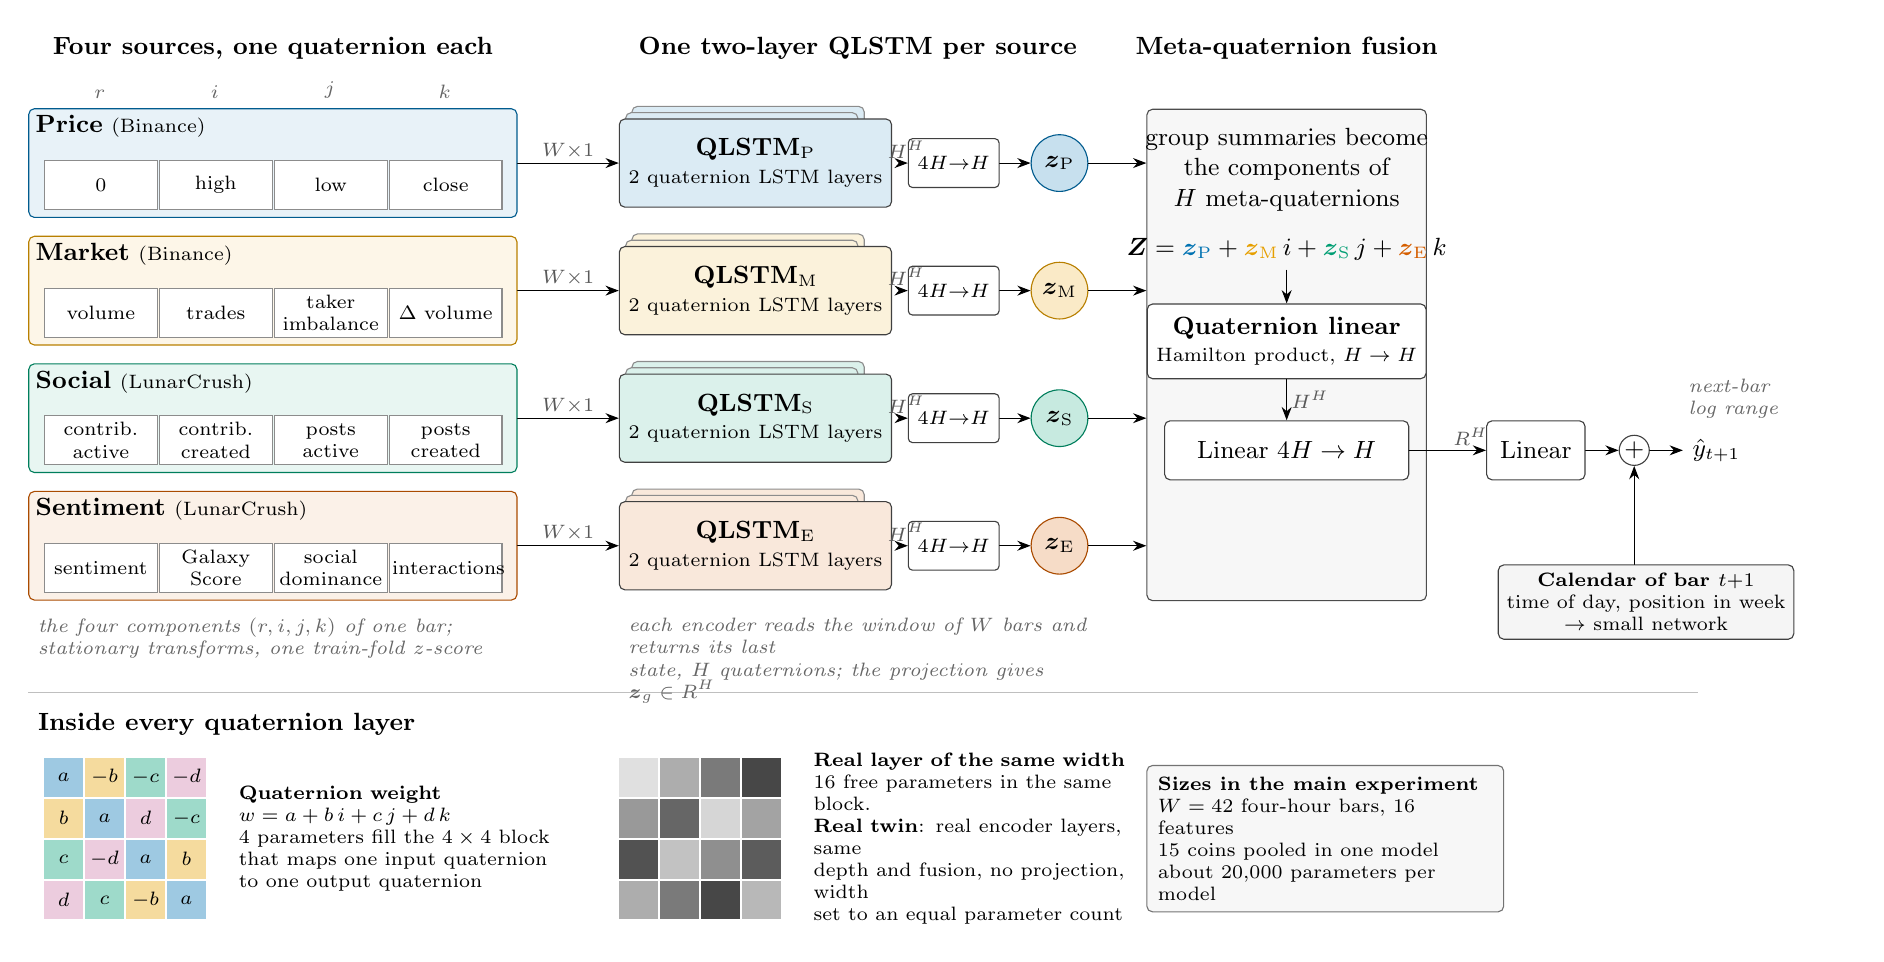
\begin{tikzpicture}[
  font=\small, >=Stealth, line cap=round,
  stage/.style={font=\bfseries\small, anchor=south},
  cell/.style={draw=black!45, fill=white, minimum width=1.42cm, minimum height=0.62cm, inner sep=1pt,
               font=\scriptsize, align=center, text width=1.36cm},
  comp/.style={font=\scriptsize\itshape, text=black!60},
  note/.style={font=\scriptsize\itshape, text=black!60, align=flush left, anchor=north west},
  blk/.style={draw=black!70, rounded corners=2pt, fill=black!4, align=center, inner sep=3pt},
  shp/.style={font=\scriptsize, text=black!65, inner sep=1.5pt},
  wcell/.style={draw=white, line width=0.8pt, minimum size=0.52cm, inner sep=0pt, font=\scriptsize}]

% ---------------------------------------------------------------- stage 1: sources -> one quaternion per group
\foreach \g/\name/\src/\col/\y/\a/\b/\c/\d in {
  P/Price/Binance/cP/0/{$0$}/{high}/{low}/{close},
  M/Market/Binance/cM/-1.62/{volume}/{trades}/{taker imbalance}/{$\Delta$ volume},
  S/Social/LunarCrush/cS/-3.24/{contrib. active}/{contrib. created}/{posts active}/{posts created},
  E/Sentiment/LunarCrush/cE/-4.86/{sentiment}/{Galaxy Score}/{social dominance}/{interactions}} {
  \node[draw=\col!80!black, rounded corners=2pt, fill=\col!9, minimum width=6.20cm, minimum height=1.38cm,
        anchor=west] (g\g) at (0,\y) {};
  \node[anchor=north west, font=\small, inner sep=2.5pt] at (g\g.north west) {\textbf{\name} {\scriptsize(\src)}};
  \foreach \k/\txt in {0/\a,1/\b,2/\c,3/\d}
    \node[cell, anchor=south west] at ($(g\g.south west)+(0.20+\k*1.46,0.10)$) {\txt};
}
\foreach \k/\lab in {0/r,1/i,2/j,3/k}
  \node[comp, anchor=south] at ($(gP.north west)+(0.91+\k*1.46,0.0)$) {$\lab$};
\node[stage] at ($(gP.north)+(0,0.50)$) {Four sources, one quaternion each};
\node[note, text width=6.1cm] at ($(gE.south west)+(0,-0.10)$)
  {the four components $(r,i,j,k)$ of one bar;\\stationary transforms, one train-fold $z$-score};

% ---------------------------------------------------------------- stage 2: group encoders
\foreach \g/\col/\y in {P/cP/0, M/cM/-1.62, S/cS/-3.24, E/cE/-4.86} {
  \foreach \o in {0.16,0.08}
    \node[draw=black!45, rounded corners=2pt, fill=\col!14, minimum width=2.95cm, minimum height=1.12cm,
          anchor=west] at ($(7.50,\y)+(\o,\o)$) {};
  \node[draw=black!75, rounded corners=2pt, fill=\col!14, minimum width=2.95cm, minimum height=1.12cm,
        anchor=west, align=center] (e\g) at (7.50,\y) {\textbf{QLSTM$_{\mathrm{\g}}$}\\[-1pt]{\scriptsize 2 quaternion LSTM layers}};
  \node[draw=black!75, rounded corners=1.5pt, fill=white, minimum width=0.95cm, minimum height=0.62cm,
        anchor=west, font=\scriptsize] (p\g) at (11.17,\y) {$4H{\to}H$};
  \node[draw=\col!80!black, circle, fill=\col!22, minimum size=0.72cm, inner sep=0pt, anchor=west]
        (z\g) at (12.73,\y) {$\bm{z}_{\mathrm{\g}}$};
  \draw[->] (g\g.east) -- node[shp, above] {$W{\times}1$} (e\g.west);
  \draw[->] ($(e\g.east)+(0.16,0)$) -- node[shp, above] {$\mathbb{H}^{H}$} (p\g.west);
  \draw[->] (p\g.east) -- (z\g.west);
}
\node[stage] at ($(eP.north |- gP.north)+(1.3,0.50)$) {One two-layer QLSTM per source};
\node[note, text width=6.0cm] at ($(eE.south west |- gE.south west)+(0,-0.10)$)
  {each encoder reads the window of $W$ bars and returns its last\\state, $H$ quaternions; the projection gives $\bm{z}_g\in\mathbb{R}^{H}$};

% ---------------------------------------------------------------- stage 3: meta-quaternion fusion
\node[blk, minimum width=3.55cm, minimum height=6.24cm, anchor=north west, fill=black!3]
  (fus) at (14.20,0.69) {};
\node[anchor=north, font=\small, align=center] (ft) at ($(fus.north)+(0,-0.12)$)
  {group summaries become\\the components of\\$H$ meta-quaternions};
\node[anchor=north, font=\small] (fz) at ($(ft.south)+(0,-0.10)$)
  {$\bm{Z}=\textcolor{cP}{\bm{z}_{\mathrm{P}}}+\textcolor{cM}{\bm{z}_{\mathrm{M}}}\,i
     +\textcolor{cS}{\bm{z}_{\mathrm{S}}}\,j+\textcolor{cE}{\bm{z}_{\mathrm{E}}}\,k$};
\node[draw=black!75, rounded corners=2pt, fill=white, minimum width=3.1cm, minimum height=0.95cm,
      align=center, anchor=north] (fq) at ($(fz.south)+(0,-0.42)$)
  {\textbf{Quaternion linear}\\[-1pt]{\scriptsize Hamilton product, $H\to H$}};
\node[draw=black!75, rounded corners=2pt, fill=white, minimum width=3.1cm, minimum height=0.75cm,
      align=center, anchor=north] (fl) at ($(fq.south)+(0,-0.52)$) {Linear $4H\to H$};
\draw[->] (fz.south) -- (fq.north);
\draw[->] (fq.south) -- node[shp, right] {$\mathbb{H}^{H}$} (fl.north);
\foreach \g in {P,M,S,E} \draw[->] (z\g.east) -- (z\g.east -| fus.west);
\node[stage] at ($(fus.north |- gP.north)+(0,0.50)$) {Meta-quaternion fusion};

% ---------------------------------------------------------------- stage 4: output
\node[draw=black!75, rounded corners=2pt, fill=white, minimum width=1.25cm, minimum height=0.75cm,
      anchor=west] (head) at ($(fus.east |- fl.east)+(0.75,0)$) {Linear};
\node[draw=black!75, circle, fill=white, inner sep=0.5pt, anchor=west] (plus) at ($(head.east)+(0.42,0)$) {$+$};
\node[anchor=west, align=left] (yh) at ($(plus.east)+(0.42,0)$) {$\hat y_{t+1}$};
\node[note, text width=2.0cm, anchor=south west] at ($(yh.north west)+(-0.05,0.02)$) {next-bar\\log range};
\node[draw=black!75, rounded corners=2pt, fill=black!4, align=center, anchor=north, inner sep=3pt, font=\scriptsize]
      (cal) at ($(plus.south)+(0.15,-1.25)$) {\textbf{Calendar of bar $t{+}1$}\\time of day, position in week\\$\to$ small network};
\draw[->] (cal.north -| plus.south) -- (plus.south);
\draw[->] (fl.east) -- node[shp, above, pos=0.80] {$\mathbb{R}^{H}$} (head.west);
\draw[->] (head.east) -- (plus.west);
\draw[->] (plus.east) -- (yh.west);

% ---------------------------------------------------------------- inset: what a quaternion layer shares
\begin{scope}[shift={(0.0,-7.75)}]
  \node[anchor=west, font=\bfseries\small] at (0,0.62) {Inside every quaternion layer};
  % Hamilton block of one weight quaternion w = a + b i + c j + d k (map x -> x (x) w)
  \foreach \r/\row in {0/{wa/a,wb/{-b},wc/{-c},wd/{-d}}, 1/{wb/b,wa/a,wd/d,wc/{-c}},
                       2/{wc/c,wd/{-d},wa/a,wb/b}, 3/{wd/d,wc/c,wb/{-b},wa/a}} {
    \foreach \col/\txt [count=\ci from 0] in \row
      \node[wcell, fill=\col!38] at (0.45+\ci*0.52,-0.05-\r*0.52) {$\txt$};
  }
  \node[anchor=west, align=left, text width=4.3cm, font=\scriptsize] at (2.55,-0.83)
    {\textbf{Quaternion weight}\\$w=a+b\,i+c\,j+d\,k$\\4 parameters fill the $4\times4$ block\\that maps one input quaternion\\to one output quaternion};
  % real twin: 16 free weights
  \foreach \r in {0,1,2,3} \foreach \ci in {0,1,2,3} {
    \pgfmathtruncatemacro{\shade}{12+mod(\r*7+\ci*5,16)*4}
    \node[wcell, fill=black!\shade] at (7.75+\ci*0.52,-0.05-\r*0.52) {};
  }
  \node[anchor=west, align=left, text width=4.2cm, font=\scriptsize] at (9.85,-0.83)
    {\textbf{Real layer of the same width}\\16 free parameters in the same block.\\\textbf{Real twin}: real encoder layers, same\\depth and fusion, no projection, width\\set to an equal parameter count};
  \node[draw=black!55, rounded corners=2pt, fill=black!3, anchor=west, align=flush left, text width=4.25cm,
        font=\scriptsize, inner sep=4pt] at (14.20,-0.83)
    {\textbf{Sizes in the main experiment}\\$W=42$ four-hour bars, 16 features\\15 coins pooled in one model\\about 20{,}000 parameters per model};
\end{scope}
\begin{scope}[on background layer]
  \draw[black!25, line width=0.4pt] (0,-6.72) -- (21.2,-6.72);
\end{scope}
\end{tikzpicture}
\end{document}
